\documentclass{article}
\usepackage{tikz}
\tikzset{
  barlabels/.style={font=\footnotesize\sffamily},
  declare function={
    barheight=5pt;
  }
}
\begin{document}
\begin{center}
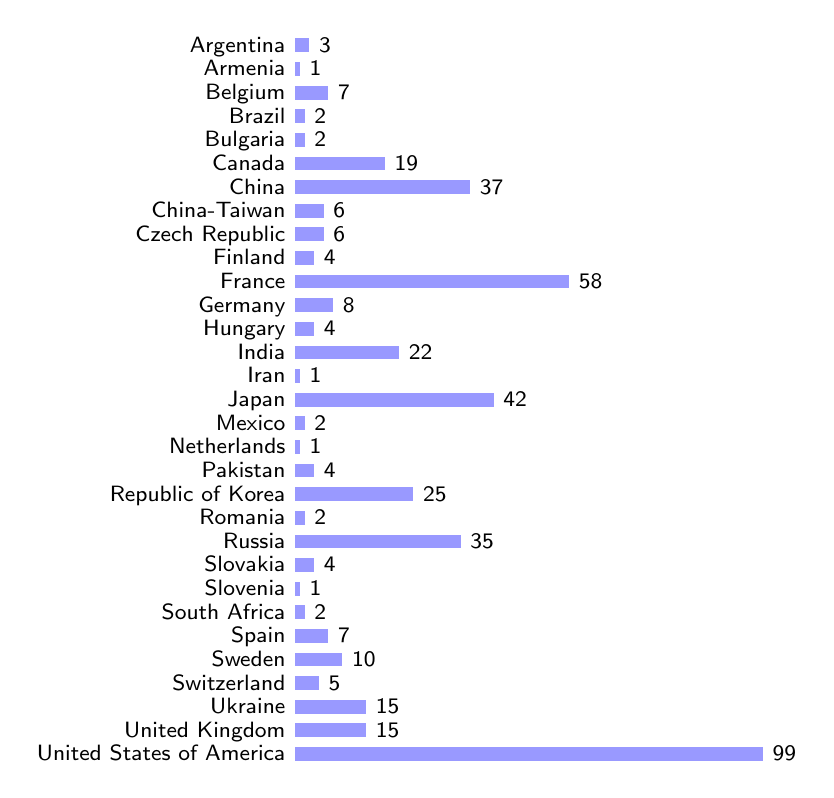
\begin{tikzpicture}[
  y=0.3cm,
  x=0.06cm,
]

\foreach [count=\i from 0] \p/\t in
                  {3/Argentina,
                   1/Armenia,
                   7/Belgium,
                   2/Brazil,
                   2/Bulgaria,
                   19/Canada,
                   37/China,
                   6/China-Taiwan,
                   6/Czech Republic,
                   4/Finland,
                   58/France,
                   8/Germany,
                   4/Hungary,
                   22/India,
                   1/Iran,
                   42/Japan,
                   2/Mexico,
                   1/Netherlands,
                   4/Pakistan,
                   25/Republic of Korea,
                   2/Romania,
                   35/Russia,
                   4/Slovakia,
                   1/Slovenia,
                   2/South Africa,
                   7/Spain,
                   10/Sweden,
                   5/Switzerland,
                   15/Ukraine,
                   15/United Kingdom,
                   99/United States of America
                   }
  {
   \node [anchor=base east,
          barlabels,
          name=i-\i] at (0,-\i) {\t};
   \fill [blue!40] (i-\i.base east) rectangle ++(\p,barheight)  ++(0,-barheight)
          node[barlabels, 
               black,
               anchor=base west] {\p};
  }

\end{tikzpicture}

\bigskip

Two columns:

\bigskip

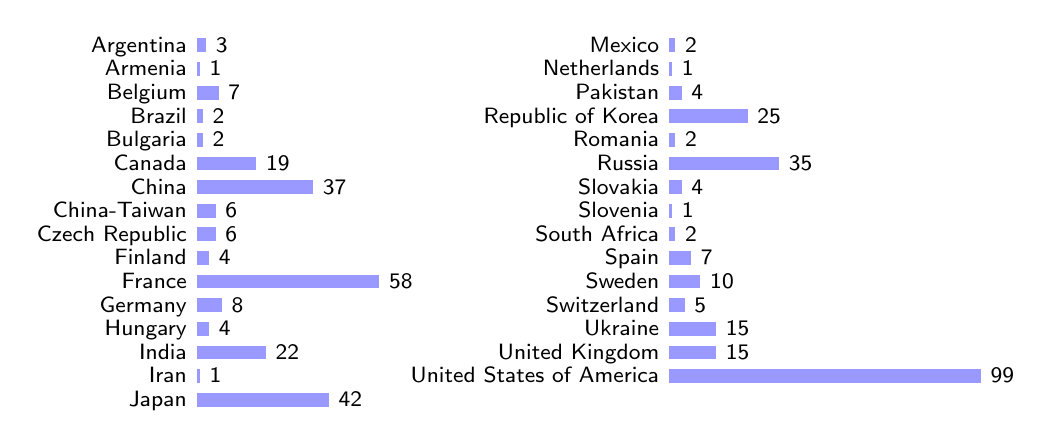
\begin{tikzpicture}[
  y=0.3cm,
  x=0.04cm,
  barlabels/.style={font=\footnotesize\sffamily}
]

\foreach [count=\i from 0] \p/\t in
                  {3/Argentina,
                   1/Armenia,
                   7/Belgium,
                   2/Brazil,
                   2/Bulgaria,
                   19/Canada,
                   37/China,
                   6/China-Taiwan,
                   6/Czech Republic,
                   4/Finland,
                   58/France,
                   8/Germany,
                   4/Hungary,
                   22/India,
                   1/Iran,
                   42/Japan,
                   2/Mexico,
                   1/Netherlands,
                   4/Pakistan,
                   25/Republic of Korea,
                   2/Romania,
                   35/Russia,
                   4/Slovakia,
                   1/Slovenia,
                   2/South Africa,
                   7/Spain,
                   10/Sweden,
                   5/Switzerland,
                   15/Ukraine,
                   15/United Kingdom,
                   99/United States of America
                   }
  {
   \node [anchor=base east,
          barlabels,
          name=i-\i] at ({ifthenelse(\i < 16,0,150)},{-mod(\i,16)}) {\t};
   \fill [blue!40] (i-\i.base east) rectangle ++(\p,barheight)  ++(0,-barheight)
          node[barlabels, 
               black,
               anchor=base west] {\p};
  }

\end{tikzpicture}
\end{center}
\end{document}

